\section{Electrostatics}
We don't have a good non-circular definition of what exactly electric charge is, but we can certainly measure it. The units of electric charge are called coulombs and denoted with a C. \\
It turns out that electric charge is quantized, meaning that it comes in discrete amounts. Any amount of electric charge comes in integer multiples of the fundamental unit of charge $e$, which is measured to be $e$ = 1.60 $\cdot$ 10$^{-19}$ C. This is a really small number - so small, in fact, that we effectively treat charge as a continuous quantity that can take on any real value. Clearly, this is not true - but the macroscopic quantities of charge that we will work with will basically behave as if charge were continuous. This means that we can use calculus and the math we used in mechanics, even with the knowledge that particles carry strictly integer amounts of the fundamental unit of charge (even if they are very large integers). \\
Charges can be positive, negative, or zero. Regardless of what value we assign to the charge because we will generally be deriving formulas in terms of a variable representing the charge, the math will still turn out the same. Therefore, there isn't really a need to rederive all the formulas that we need for negative charges as well as for positive ones because they should be the same depending on what value we plug in. However, qualitatively, we will just assume charges are positive to get a feel for how the formulas work.\\
Before studying charges in motion, we will first discuss the behaviors and interactions of stationary charges. This study is called electrostatics and is the foundation upon which we will build our knowledge of electromagnetism. 
\subsection{Coulomb's Law}
We first must answer the question: How does charge interact with itself? We already probably know that charges with the same sign repel each other, and charges with differing signs attract, as observed in nature. This force also should decrease in magnitude as the distance between the charges increases - after all, if you move oppositely charged things really far away from each other, there doesn't appear to be an observable force between them, whereas a much more observable one appears once the charges are close enough. A clever scientist by the name of Charles-Augustin de Coulomb came up with his self-named law that describes the electric force between two charges $q_1$ and $q_2$, using macroscopic observations. If $r_{12}$ is the distance between these charges, and the unit vector $\hat r_{12}$ is the unit vector that points from charge $q_1$ in the direction of $q_2$, we have that the force exerted on charge $q_2$ by $q_1$ is:
\[
	\vec F = \frac{kq_1q_2}{r_{12}^2} \hat r_{12}
\]
\begin{center}
    \begin{asy}
        import geometry;
        size(8cm);
        
        draw(unitcircle);
        draw(shift(15, 0) * unitcircle);
        draw((-1,0)--(-3,0), Arrow);
        draw((16,0)--(18,0), Arrow);
        
        draw((0, -1.5)--(15, -1.5), linetype("8 8"), Arrows);
        
        label("$q_1$", (0, 1), N);
        label("$q_2$", (15, 1), N);
        label("$r_{12}$", (0, -1.5)--(15, -1.5), S);
        label("$\vec F_{12}$", (-1,0)--(-3,0), N);
        label("$\vec F_{21}$", (16,0)--(18,0), N);
    \end{asy}
\end{center}
Notice how this is also an inverse-square law, just like the force of gravity - in fact, it's essentially the same, up to a sign and the proportionality constant, $k$. In this case, $k$ is Coulomb's constant, and has been measured to be 8.99 $\cdot$ 10$^9$ N $\cdot$ m$^2$/C$^2$. Sometimes, we will see Coulomb's Law written in the following manner:
\[
	\vec F = \frac{1}{4 \pi \epsilon_0} \frac{q_1q_2}{r_{12}^2} \hat r_{12}
\]
where the $k$ has been replaced with $\frac{1}{4 \pi \epsilon_0}$. These expressions are the same, except now our proportionality constant is written in terms of $\epsilon_0$, called the permeability of free space. This has a value of 8.85 $\cdot$ 10$^{-12}$ C$^2$/(N $\cdot$ m$^2$), and it'll come up often in place of $k$ (for reasons we will discuss later). 
\subsection{Electric Fields and Superposition}
When we introduced the gravitational force, we also introduced the gravitational field, which assigned a vector to every point in space that represented the force done per unit mass. We can do something similar for the electric force. For a charge $q_0$, and a net electric force on this particle $\vec F_{net}$, we have that the electric field at this point $\vec E$ is:
\[
	\vec E = \frac{\vec F}{q_0}
\]
Just like with gravity, we will have to calculate the electric field not just for collections of point charges, but also for continuous distributions of charge. Because of the similarity between the gravitational and electric forces, all of the formulas derived using superposition of forces and fields in the gravity section essentially apply to electrostatics. We can follow the same logic employed there to arrive at the electric field on the axis of a uniform ring of change, and the electric field due to a thin spherical shell of charge:
\[
	\text{Ring: } \vec E = \frac{kQy}{(R^2 + y^2)^{3/2}}\hat y \quad \text{Spherical Shell, outside: } \vec E = \frac{kQ}{r^2}\hat r \quad \text{Spherical Shell, inside: } \vec E = 0
\]
We're going to calculate two more fields here - one being the field due to an infinite line charge, and the other the field of an infinite plane charge. \\
For the infinite line charge, we can assume it's uniform with linear charge density $\lambda$ and we can parameterize it using the real number line. For simplicity, we'll place a test charge $q_0$ radially outward from the line a distance of $y$ away at $x$-coordinate $x=0$.\\
\begin{center}
    \begin{asy}
        import geometry;
        size(9cm);
        
        real y = 5;
        dot((0, y));

        draw((0,0)--(-10,0), linetype("4 4"), Arrow);
        draw((0,0)--(10,0), linetype("4 4"), Arrow);
        draw((-4.25,0)--(0,y), linetype("6 6"));
        draw((0, y)--(0,0));
        draw((-4,0)--(-4.5,0), linewidth(2));

        label("$y$", (0, y/2), dir(0));
        label("$x$", (-2, -0.5), dir(270));
        label("$dx$", (-4.25, -0.5), dir(270)*0.2);
        label("$q_0$", (0, y), dir(130));
    \end{asy}
\end{center}
Consider now an infinitesimal subdivision of the line with length $dx$ and at coordinate $x$. The charge of this point is $dq = \lambda \, dx$, and we can use Coulomb's Law to figure out the force on the test charge:
\[
	dF = \frac{kq_0\, dq}{x^2 + y^2}
\]
This, however, is the magnitude of the force - we haven't taken into consideration that all the components in the $x$-direction will cancel, by symmetry. Therefore, we have to project into the radial direction and find the $r$-component of the force, where the $r$-direction is radially outward from the cylindrical symmetry of the wire. 
\[
	dF_r = \frac{kq_0 \, dq \, y}{(x^2 + y^2)^{3/2}}
\]
The electric field due to the small portion of the wire is then:
\[
	dE_r = \frac{k\lambda y \, dx}{(x^2+y^2)^{3/2}}
\]
We now have to integrate over all these portions of wire, from $-\infty$ to $\infty$:
\begin{align*}
	E &= \int_{-\infty}^{\infty} \frac{k\lambda y \, dx}{(x^2+y^2)^{3/2}}\\
	&= k\lambda y  \int_{-\infty}^{\infty} \frac{dx}{(x^2+y^2)^{3/2}}
\end{align*}
We can make the clever $u$-substitution $x = y \tan u$, $dx = y \sec^2 u \, du$. This means the bounds of the integral change to $-\frac{\pi}{2}$ to $\frac{\pi}{2}$:
\begin{align*}
	E &= k\lambda y  \int_{-\infty}^{\infty} \frac{dx}{(x^2+y^2)^{3/2}} \\
	&= k \lambda y \int_{- \frac{\pi}{2}}^{\frac{\pi}{2}} \frac{y \sec^2 u \, du}{(y^2 \tan^2 u + y^2)^{\frac{3}{2}}}\\
	&= k \lambda y^2 \int_{- \frac{\pi}{2}}^{\frac{\pi}{2}} \frac{\sec^2 u \, du}{(y^2 \sec^2 u)^{\frac{3}{2}}} \\
	&= k \lambda y^2 \int_{- \frac{\pi}{2}}^{\frac{\pi}{2}} \frac{\sec^2 u du}{y^3 \sec^3 u} \\
	&= \frac{k \lambda}{y} \int_{- \frac{\pi}{2}}^{\frac{\pi}{2}} \frac{\sec^2 u \, du}{\sec^3 u}\\
	&= \frac{k \lambda}{y} \int_{- \frac{\pi}{2}}^{\frac{\pi}{2}} \cos  u \, du \\
	&= \frac{2 k \lambda}{y}
\end{align*}
And all is well in the end, as the integral collapses into a simple form.\\
We can now use a superposition of these infinite lines to find the electric field for a uniform plane of charge with surface charge density $\sigma$. Let's orient the plane of charge with the $xy$-plane, and put a test charge $q_0$ at a point a distance $z$ above the origin. \\
\begin{center}
    \begin{asy}
        import three;
        size(8cm);
        
        triple eye = (0.6, 1, 0.4);
        currentprojection = orthographic(eye);
        
        real planesize = 2.5, z = 0.3;
        
        real ps = planesize/2;
        draw((ps, ps, 0)--(-ps, ps, 0)--(-ps, -ps, 0)--(ps, -ps, 0)--cycle);
        draw((ps * X)--(1.4 * ps * X), dashed, EndArrow3);
        draw((-ps * X)--(-1.4 * ps * X), dashed, EndArrow3);
        draw((ps * Y)--(1.4 * ps * Y), dashed, EndArrow3);
        draw((-ps * Y)--(-1.4 * ps * Y), dashed, EndArrow3);
        
        dot(z * Z);
        draw(O--(z * Z));
        label("$z$", z/2 * Z, dir(180));
    \end{asy}
\end{center}
We can consider lines of charge parallel to the $y$-axis and with charge density $\lambda = \sigma \, dx$. With this, we can determine the magnitude of the electric field on the point by each line charge $dF$:
\[
	dE = \frac{2k\sigma \, dx}{\sqrt{x^2 + z^2}}
\]
Since the plane has rotational symmetry, there should only be a $z$-component of the electric field, so we can only consider the projections of the electric field in that direction:
\[
	dE_z = \frac{2k\sigma z \, dx}{x^2 + z^2}
\]
We can integrate from $-\infty$ to $\infty$ again across all the line charges, and obtain:
\begin{align*}
	E_z &= \int_{-\infty}^{\infty} \frac{2k\sigma z \, dx}{x^2 + z^2}\\
	&= \frac{2k\sigma}{z} \int_{-\infty}^{\infty} \frac{dx}{1 + \left(\frac{x}{z}\right)^2 } \\
	&= \frac{2k\sigma}{z} \int_{-\infty}^{\infty} \frac{z \, du}{1 + u^2}\\
	&= 2k\sigma \arctan u \Big|_{-\infty}^{\infty}\\
	&= 2k\pi \sigma = \frac{\sigma}{2\epsilon_0}
\end{align*}
Notice that this is independent of $z$. The infinite plane charge will be the most common uniform electric field that we will study, and will be directed out of the plane for positive charge density and into the plane for negative charge density. \\
The principle of superposition with Coulomb's Law can be used to derive a number of electric fields, and it is important that you know how to come up with these derivations. \\
It's also important that you can draw (to a limited extent) how the electric field looks in space. To do this, we use field lines, which show the direction of the electric field and also show how it flows around objects. It's also important to note that the field lines trace out the forces on a positively charged particle if it was just left in space. We sometimes limit the number of field lines we draw to a few, but space them out the weaker the field is around a region. As an example, we can look at the case for an electric dipole:
\begin{center}
	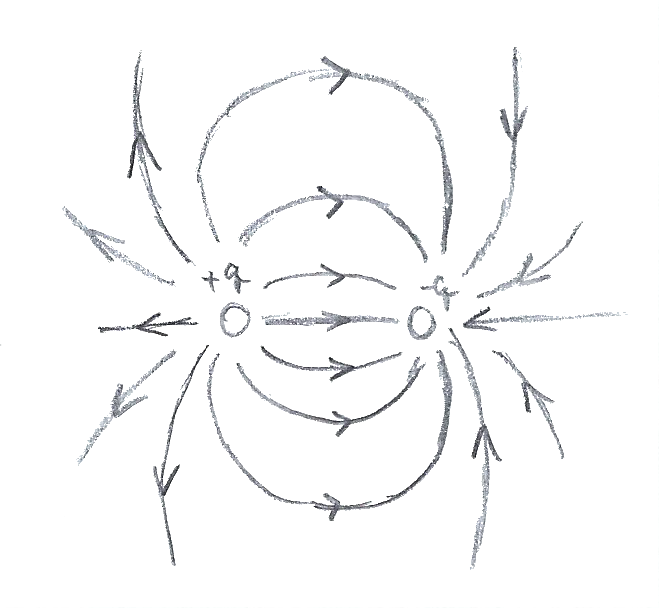
\includegraphics[scale=0.3]{images/em/dipolefield.png}
\end{center}
We will look at the fields of a dipole and its behavior in the problems. 
\subsection{Gauss' Law for Electric Fields}
It turns out that while the principle of superposition is good for finding the electric field, there is an easier way to do so in some symmetric cases. First, we have to talk about the flux of a vector field through a surface. For a flat surface with area $A$, a normal vector to the surface $\hat n$, and a vector field (in this case, the electric field $\vec E$), we have that the flux $\Phi$ through this surface is:
\[
	\Phi = \vec E \cdot \hat n \cdot A
\]
\begin{center}
	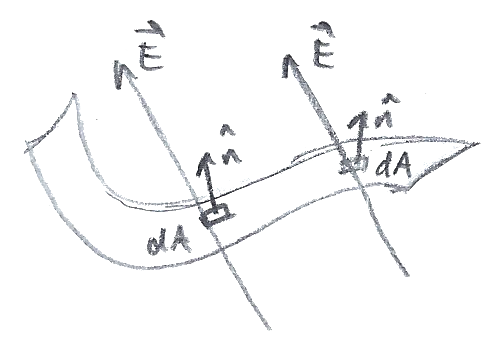
\includegraphics[width=0.3\textwidth]{images/em/electricflux.png}
\end{center}
As you can see from the formula, the flux is a scalar quantity that more or less describes how much a field is flowing through a surface. If the surface in question is not flat, we have to subdivide the surface into many extremely small pieces of area $dA$ that are approximately flat and let the number of pieces go to infinity. We can then calculate the flux $d\Phi$ through each piece:
\[
	d\Phi = \vec E \cdot \hat n \, dA
\]
If we add up all these small amounts of flux, this is what's called a  surface integral, and the flux through some surface $S$ is written as:
\[
	\Phi = \int_S \vec E \cdot \hat n \, dA
\]
If the surface happens to be closed (like a bubble-kind of thing), we draw a circle on the integral sign:
\[
	\Phi = \oint_S \vec E \cdot \hat n\, dA
\]
It's worth mentioning that for closed surfaces (also called Gaussian surfaces) we usually choose the normal vectors to be on the outside or, side of the surface that doesn't have finite volume. (But I'm sure you all know what "outside" means, hopefully, even if you don't go there.)\\
Gauss' Law deals with the electric flux $\Phi_E$ through a closed surface $S$. Specifically, the claim is that the electric flux through a closed surface is proportional to the charge enclosed, written quantitatively as:
\[
	\Phi_E = \oint_S \vec E \cdot \hat n \, dA = \frac{Q_{inside}}{\epsilon_0}
\]
The proportionality constant $\epsilon_0$ is the same one that showed up in Coulomb's constant $k$. \\
Usually, it's impractical to evaluate the surface integral on the left -hand side, so Gauss' Law is usually used to figure out the distributions of charge if the electric field is known. For symmetric cases, however, the flux through some carefully chosen closed surfaces is easy to evaluate, so we can actually derive some electric fields in this manner. Consider first a single charged particle of charge $q$, and say we wish to find the electric field a distance $r$ away from it. We can construct a Gaussian sphere (indicated with the dotted line) with radius $r$ around the particle, and notice that by symmetry, the electric field has to be spherically symmetric and have the same magnitude at the same distances away from the charged particle. \\
\begin{center}
	\begin{asy}
		import graph;
        size(4cm);
        draw(Circle((0, 0), 0.2));
        dot((0,0));
        draw((0,0)--(1.5, 0));
        dot((1.5, 0));
        draw(Circle((0, 0), 1.5), linetype("4 4"));

        label("$q$", dir(60)*0.2, dir(120));
        label("$r$", (0,0)--(1.5,0), dir(90));
	\end{asy}
\end{center}
From this, we can compute the flux as the surface area of the surface times the electric field, or:
\[
	\Phi_E = E \cdot 4 \pi r^2 = \frac{q}{\epsilon_0}
\]
From this we obtain:
\[
	\vec E = \frac{1}{4\pi\epsilon_0} \cdot \frac{q}{r^2} \hat r = \frac{kq}{r^2} \hat r
\]
This is consistent with Coulomb's Law, so Gauss' Law fits in our current framework for electric fields. It turns out that if we run this logic backwards, in a sense, we can also show that Coulomb's Law implies Gauss' Law. \\
In general, though, it still isn't clear that we can apply this to any sort of surface. It turns out that for any convex surface, we can map a sphere to this new convex surface by projecting each patch of area on the sphere to one on the new surface. The flux remains the same through this new patch of area because even though the area of the patch might fluctuate or change based on the square of the distance to the dilation point, the electric field will compensate because it also follows an inverse-square law. Because of this, the size of the convex surface doesn't matter. Furthermore, no charge outside of the surface will contribute anything to the flux, because all the flux of the electric field going into the surface must eventually have the same amount leaving the surface, due to this proportionality. Therefore, it's feasible to have any sort of shape work, even though we won't necessarily be able to use it.\\
There are some special cases that yield easily to Gauss' Law. Let's revisit the infinite line charge with charge density $\lambda$. \\
\begin{center}
    \begin{asy}
        import solids;
        import three;
        size(8cm);
        draw((1, 1, 1)--(0, 1, 1), EndArrow3);
        draw((2, 1, 1)--(3, 1, 1), EndArrow3);
        draw((2, 1, 1)--(1, 1, 1), linetype("2 4"));
        currentprojection=orthographic(0.7, 1, 1);
        currentlight=nolight;
        triple start = (1,1,1);
        real length = 1;
        real radius = 0.5;
        triple ax = (1,0,0);
        revolution r = cylinder(start,radius,length,ax);
        draw(r,black);
        
        draw((2, 1, 1)--(2, 1, 1.5), grey);
        label("$y$", (2, 1, 1.25), dir(180)); 
        draw((2, 2, 1)--(1, 2, 1), linetype("8 8"), EndArrow3);
        draw((1, 2, 1)--(2, 2, 1), linetype("8 8"), EndArrow3);
        label("$L$", (1.5, 2, 1), dir(315)); 
    \end{asy}
\end{center}
Consider a Gaussian cylinder that has its axis of symmetry as the line with length $L$ and radius $y$. The charge enclosed is then $\lambda \cdot L$. Because by symmetry the electric field has to point radially outward, the only flux has to be through the curved side of the cylinder, as no electric field lines pass through the two sides of the cylinder. Furthermore, we know the line of charge should have the same magnitude for the electric field at the same distance from the line charge. With this in mind, we can apply Gauss' Law:
\[
	\oint_S \vec E \cdot \hat n \, dA = E \cdot 2 \pi y L = \frac{\lambda L}{\epsilon_0}
\]
Notice how the $L$ cancels from both sides, leaving us with the electric field:
\[
	E = \frac{\lambda}{2\pi y \epsilon_0} = \frac{2k\lambda}{y}
\]
With Gauss' Law, we can drastically reduce the computation needed for electric fields for symmetric cases, although we do have to be somewhat careful or inventive to deal with these cases. \\ 
\subsection{Electric Potential}
As we discussed when studying mechanics, gravity has a potential energy function and is a conservative force. It turns out that the electromagnetic force is also conservative and has a very similar potential energy function. For a point charge $q$, and assuming the potential energy is zero infinitely far away, we have the potential energy of another charge $q_0$ to be:
\[
	U(r) = -\int_C \vec F \cdot d\vec r = \int_r^{\infty} \frac{kqq_0}{r^2} \, dr = \frac{kqq_0}{r}
\]
Similar to what we did for electric fields, we can define the electric potential $V(r)$ of a charge $q_0$ as the potential energy per unit charge, measured in volts (V):
\[
	V(r) = \frac{U(r)}{q_0} = \frac{kq}{r}
\]
Because of the same division by a charge that we did for electric fields, we can relate the electric field and the electric potential by the following:
\[
	\Delta V = \frac{\Delta U}{q_0} = -\frac{1}{q_0}\int_C \vec F \cdot \, d\vec r = - \int_C \frac{\vec F}{q_0} \cdot d\vec r = -\int_C \vec E \cdot d\vec r
\]
Therefore, we can take the line integral of the electric field to find the potential. Be careful to distinguish between potential energy and potential - potential is energy per unit charge, and is not the same as potential energy, even if their names make it sound like they are the same. \\
Potential follows the principle of superposition as well, but because it is a scalar, there is no need to consider the "direction" of the electric field other than when taking the dot product. For an example, we can revisit the potential of a ring of charge of radius $R$, charge $Q$, and uniform linear charge density $\lambda = \frac{Q}{2\pi R}$. \\
\begin{center}
    \begin{asy}
        import three;
        size(6cm);
        
        triple eye = (7, 8, 5);
        currentprojection = perspective(eye);
        
        triple center = (0, 0, 0);
        real R = 1, y = 2;
        
        draw(circle(center, R, Z));
        dot((0, 0, y));
        
        real dqAngle = -20, dqDelta = 6;
        draw(arc(center, R,
                90, dqAngle - dqDelta,
                90, dqAngle + dqDelta), linewidth(2));
        
        draw(dir(90, dqAngle) -- (0, 0, y), linetype("6 6"));
        
        triple radiusPt = R * dir(90, 170);
        draw((0, 0, 0)--radiusPt, gray(0.2));
        draw((0, 0, 0)--(0, 0, y), gray(0.2));
        
        label("$Q$", (0, R, 0), dir(-90));
        label("$q_0$", (0, 0, y), dir(130));
        label("$dQ$", dir(90, dqAngle), dir(200));
        label("$R$", radiusPt/2, dir(-40));
        label("$y$", (0, 0, y/2), dir(0));
    \end{asy}
\end{center}
For a small arc of the ring, recall that the charge on this portion $dQ = \lambda R \, d\theta$, so the potential $dV$ at a point a distance $y$ above the center of the ring is:
\[
	dV = \frac{k\, dQ}{\sqrt{R^2+y^2}} = \frac{k\lambda R \, d\theta}{\sqrt{R^2+y^2}}
\]
If we integrate with respect to $\theta$ from $0$ to $2\pi$, the integral evaluates to:
\[
	V = \frac{kQ}{\sqrt{R^2+y^2}}
\]
It's important to be able to derive the potentials of the electric fields easily - a table of them for common charge configurations is included at the end. \\
We can also visualize the potential graphically as we did for electric fields. Usually, this is done by drawing a curve connecting all the places where the potential is the same. These lines are called equipotential lines, or if we're in 3-D space, equipotential surfaces. As an example, the blue lines are the equipotentials for the dipole field:
\begin{center}
	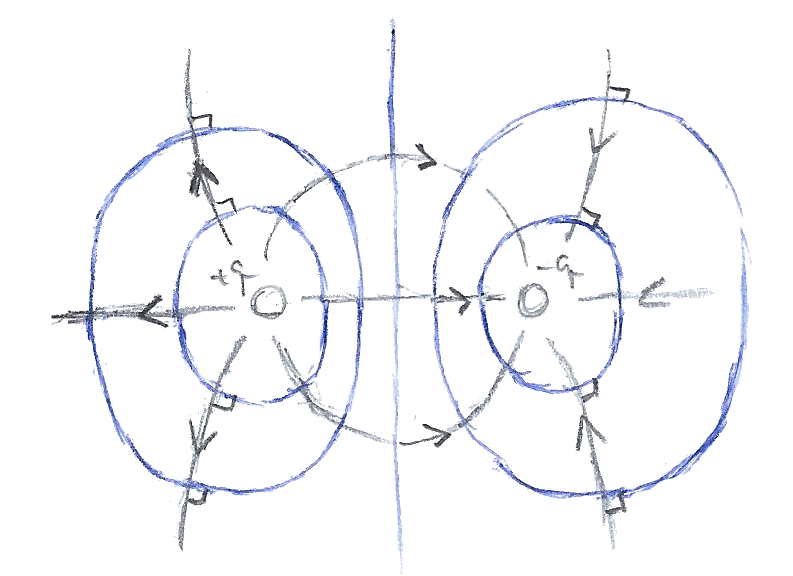
\includegraphics[scale=0.3]{images/em/equipotentials.png}
\end{center}
At equipotentials, the electric force will do no work on the particle as it travels on the surface. Since the electric field points in the direction of the force that does work to push charged particles to lower potentials as well, we can also draw the electric field lines based on equipotential diagrams. 
\subsection{Summary and Problems}
Electrostatics is a huge unit, where we talked about electric charges, fields, potentials, and flux. We first looked at how the electric force between charged objects obeyed an inverse square law, like gravity. We have a lot of tools to look at how stationary electric charges produce electric fields and exert a force on each other - one of our tools is Gauss' Law, a powerful result relating the charge inside a surface to the flux of the field through it. Another powerful tool is the concept of superposition, where we know that electric fields obey vector addition, and we exploited this to find the electric fields of infinitely large/charged objects. We also were able to see that the electric field and force are conservative, and defined potential energy and potential similar to what we did for gravity. The following problems will hopefully try to address all the topics we covered in this unit as well as a little bit of a throwback to mechanics. \\

\noindent \textbf{Problems:}\\
1. (2 $\bigstar$) Two tiny conducting balls of identical mass $m$ and identical charge $q$ hang from nonconducting threads of length $L$, both at an angle $\theta$ to the vertical and from the same point. Assume $\theta$ is so small such that $\tan \theta \approx \sin \theta$. Show that the equilibrium separation of the two balls $x = \left( \frac{q^2L}{2\pi\epsilon_0 mg}\right)^{1/3}$.\\
2. (2 $\bigstar$) A dumbbell consisting of two identical small particles, each of mass $m$, is attached to the ends of a thin (massless) rod of length $a$ that has a pivot at its center. The particles have charges of $+q$ and $-q$, and the dumbbell is located in a uniform horizontal electric field of magnitude $E$, displaced an angle $\theta$ from the horizontal. Show that for small values of the angle $\theta$ between the direction of the dipole and the direction of the electric field, the system displays a rotational form of simple harmonic motion, and show that the period of that motion is $\pi \sqrt{\frac{2ma}{qE}}$. \\
3. (3 $\bigstar$, $\spadesuit$) A thin hemispherical shell of radius $R$ has a uniform surface charge $\sigma$. Show that the magnitude of the electric field at the center of the base of the hemispherical shell is $k\pi\sigma$.\\
4. (4 $\bigstar$) Two positive point charges of charge $+q$ are on the $y$-axis at $y=+a$ and $y=-a$. A bead of mass $m$ and charge $-q$ slides without friction along a taut thread that runs along the $x-$axis. Let $x$ be the position of the bead. a) Show that for $x<<a$, the bead experiences a linear restoring force (a force that is proportional to $x$ and directed toward the equilibrium position at $x=0$) and therefore undergoes simple harmonic motion. b) Show the period of the motion is $2\pi \sqrt{\frac{ma^3}{2kq^2}}$.\\
5. (3 $\bigstar$, $\spadesuit$) A quantum-mechanical treatment of the hydrogen atom shows that the electron in the atom can be treated as a smeared-out distribution of negative charge of the form $\rho(r) = -\rho_0e^{-2r/a}$. Here $r$ represents the distance from the center of the nucleus and $a$ represents the first Bohr radius. Recall that the nucleus of a hydrogen atom consists of just one proton and treat this proton as a positive point charge. Show that $\rho_0 = \frac{e}{\pi a^3}$, where $e$ is the elementary charge, using the fact that the atom is neutral. \\
6. (2 $\bigstar$, $\spadesuit$) All electric dipoles (two charges, one negative and one positive of the same magnitude $q$ a distance $d$ apart) have a dipole moment $\vec p = q \vec d$, where $\vec d$ is the vector pointing from the negative charge to the positive charge. Suppose a dipole is located at a perpendicular distance $R$ from an infinitely long line charge that has a uniform linear charge density $\lambda$. Assume that the dipole moment is in the same direction as the field of the line of charge. Show that the electric force on the dipole is $\frac{2k\lambda p}{R^2}$ if $d << R$.\\
7. (1 $\bigstar$) An infinitely long nonconducting solid cylinder of radius $a$ has a uniform volume charge density of $\rho_0$. Show that the electric field a distance $R$ from the long axis of the cylinder is $E = \frac{\rho_0R}{2\epsilon_0}$ if $0\leq R < a$ and $E = \frac{\rho_0a^2}{2\epsilon_0 R}$ if $R > a$. \\
8. (2 $\bigstar$, $\spadesuit$) A nonconducting solid sphere of radius $R$ has a volume charge density that is proportional to the distance from the center $r$. That is, $\rho = Ar$ for $r < R$, where $A$ is a constant. a) Show the total charge on the sphere is $\pi AR^4$. b) Show that the electric field inside the sphere has magnitude $\frac{Ar^2}{4\epsilon_0}$ and the electric field outside the sphere has magnitude $\frac{AR^4}{4\epsilon_0 r^2}$. \\
9. (3 $\bigstar$) Show that at a point a distance $r$ from the center of a dipole with dipole moment $\vec p$ and charges of magnitude $q$ a distance $L$ apart, we have that the potential $V = \frac{kp\cos \theta}{r^2}$ if $r >> L$ and $\theta$ is the angle between the dipole and the line from the point to the center of the dipole. \\
10. (3 $\bigstar$, $\spadesuit$) Show that the potential inside a uniformly charged solid sphere is given by $V(r) = \frac{kQ}{2R}\left(3 - \frac{r^2}{R^2}\right)$ where $R$ is the radius of the sphere, $Q$ is the charge on the sphere, and $r$ is the distance from the center. (Set $V(\infty) = 0$.)\\
11. (2 $\bigstar$) Four point charges, each with charge $+nq$, are fixed at the corners of a square centered at the origin. The length of each side of the square is $2a$. A fifth particle that has a mass $m$ and a charge $+q$ is placed at the origin and
released from rest. Show that its speed when it is very far from the origin is $v = q\sqrt{\frac{4n\sqrt{2}k}{ma}}$. \\
12. (2 $\bigstar$) A uniformly charged, infinitely long line of negative charge has a linear charge density of $-\lambda$ and is located on the $z$-axis. A small positively charged particle that has a mass $m$ and a charge $q$ is in a circular orbit of radius $R$ in the $xy-$plane centered on the line of charge. Show that the particle is moving at a speed of $v = \sqrt{\frac{2kq\lambda}{m}}$.\\
13. (2 $\bigstar$, $\spadesuit$) Two coaxial conducting cylindrical shells have equal and opposite charges. The inner shell has charge $+q$ and an outer radius $a$, and the outer shell has charge $-q$ and an inner radius $b$. The length of each cylindrical shell is $L$, and $L >> b$. Show the potential difference $\Delta V$ between the two shells is $\Delta V = \frac{2kq}{L}\ln\left(\frac{b}{a}\right)$.\\
14. (3 $\bigstar$) A stationary ring of radius $a$ lies in the $yz$-plane and has a uniform positive charge $Q$. A small particle that has mass $m$ and a negative charge $-q$ is located at the center of the ring. a) Show that if $x$ is the $x$-coordinate of the point and $x<<a$, the electric field at points along the axis of the ring is $-\frac{kQx}{a^3}$. b) Show if the particle is given a small displacement in the $+x$-direction, it will perform simple harmonic motion, and show that the period of the motion is $2\pi \sqrt{\frac{ma^3}{kqQ}}$.
\pagebreak